\documentclass[10pt,conference,compsocconf,retainorgcmds]{IEEEtran}

\usepackage{hyperref}
\usepackage{graphicx}   % For figure environment
\usepackage{color}
\usepackage{natbib}
\usepackage{float}
\usepackage{cprotect}
\usepackage{tabularx}
\usepackage{multirow}
\usepackage{subcaption}
\usepackage{amsmath}
\usepackage{amssymb}
\usepackage{enumitem}

\begin{document}
\title{Twitter Sentiment Classification: Machine Learning Project 2}

\author{
  Robin Clerc, Pierre Vigier, Jacob Levy Abitbol\\
  \textit{MSc  Computer Science, EPFL, Switzerland}
}

\maketitle

\begin{abstract}
As microblogging services like Twitter are becoming
more and more influential in today’s globalized world, its facets
like sentiment analysis are being extensively studied. The sheer volume of data produced daily by its users as well as its overall availability, enable researchers to study this classification problem over massive datasets of messages or tweets. The information collected is however inherently noisy, as phenomena such as linguistic drift are known to be sped up over these social media platforms, therefore hindering the use of standard NLP tools. We present here a combined methodology overcoming some of these issues by training a model to predict whether any given tweet is more likely to contain a happy rather than a sad emoji. Specifically, we show how different pre-processing schemes and text embedding (GloVe, word2vec) methods are crucial in driving up the quality of the  predictions yielded by our models. We eventually achieve accuracies of around 86.54\% on an already pre-processed dataset of around 2.5 million labeled tweets by aggregating several approaches.
\end{abstract}








\section{Introduction}
Sentiment classification is the task of detecting whether a textual item expresses an overall positive or negative opinion in general or about a given entity (products, person, policy).
Recently, the advent of social media and publicly available communication platforms has opened up a new gate to access individual information at a massive scale. Among all available social platforms, Twitter has been regarded as the choice by default, namely thanks to the intrinsic nature of communications taking place through it and the existence of data providers that are able to supply researchers with the volume of data they require. It is therefore not surprising that interest in studying sentiment classification through this social platform has grown in recent years. We here study a variant of the original sentiment classification problem by training a model to be able to detect whether a tweet contains  a  happy or sad emoji ( ':)' and  ':('   respectively).

\section{Data Description}
 \label{sec:structure-paper}
\subsection{Data Exploration and Preprocessing: text normalization}

Our dataset consists of a large data corpus collected from the online news and social networking service, Twitter. On it, users can post and interact with messages, "tweets", restricted to 140 characters. Specifically, we are given a sentiment-labeled dataset of 2.5 million tweets, each containing exclusively a happy or sad emoji.  Class imbalance is not an issue in the provided dataset as each sentiment class contains an even number of samples to train our models on (1.25 million for each). Metadata generally contained in the tweets is here preprocessed and indicated by some user defined tag (\textless  mention\textgreater  for @user, \textless hashtag\textgreater  for \#,...).\\

When considering what kind of preprocessing to perform on our dataset, one must first acknowledge the inherently different style of communication used though this service.  Twitter posts are for instance much shorter than in any other traditional media like blogs, as they are constrained by a hard 140 character limit. This is believed to be the cause behind the high compactness and brevity of language in Twitter. Furthermore, it contains highly non-standard orthography alongside a wide range of linguistic variation leading to several non-standard spellings of the same word and hindering the use of standard NLP tools such as tokenizer or stemmers. Keeping those words makes the dimensionality of the problem high and hence the classification more difficult since each word in the text is treated as one dimension. A logical first step would then be to reduce this intrinsic variability by filtering out infrequent word occurrences.

We proceeded to use the preprocessing scheme developed by the Stanford NLP section over a corpus of 2 billions of tweets. The interest here is two-fold: on the one hand,  having trained their methods on such a large corpus enable us to have a general set of rules to deal with exceptions that we otherwise would have had to look for in our corpus. On the other hand, relying on the same preprocessing backbone will in time, allow us to use higher level features (embeddings) developed by this group and computed over their Twitter dataset. The Ruby preprocessing script was hence translated intro Python and adapted to our already tokenized and lower-case proprocessed dataset. We here list its main features:

\begin{itemize}[label={},leftmargin=*]
    \item \textbf{Contractions expanded:} As previously stated, Twitter hard character limit incentivizes the use of contraction of words that are already common in informal text communications: \textit{"I'll've" $\rightarrow$ "I will have"}. Abbreviations are also dealt with in an analogous manner.
    \item \textbf{Hashtag split:} Hashtags come in the form of one or more concatenated words preceded b the \# character. These tokens can in some cases convey additional information that might be useful to perform sentiment analysis (e.g, \#hatetrump, \#loveobama). Although tokenizing a cleansed hashtag can prove quite hard, we assumed that most hashtags are made of a single token and considered it as a given word:\textit{ \#love$\rightarrow$ love, \#savethedate $\rightarrow$ savethedate}. Preprocessing of our data unfortunately prevents us from actually using this step.
    
    \item \textbf{Spell check}: Typos naturally present in the tweets are partially corrected via the edit distance (insertion, deletion, substitution)  to standard words found in online dictionaries. The application of this filter was restricted by the correction speed and the volume of the data we were dealing with : \textit{piercin $\rightarrow$ piercing}. We also introduced some user-defined rules in order to account for frequently observed typos such as character repetitions , where characters observed more than twice are set to be repeated only twice: \textit{gooooood $\rightarrow$ good, honeeeyyy $\rightarrow$ honeeyy}
   \end{itemize}

It is also worth mentioning that some standard NLP preprocessing techniques were tried but finally excluded from the final pipeline such as stopwords removal, which was found to be decreasing the prediction accuracy, part-of-speech tagging which wasn't found to increase our final prediction score. \\
It should also be said that the order in which the preprocessing stages are concatenated is crucial to the overall performance of our model (for instance, letter repetitions should be removed before checking whether a given word is in the dictionary or not). The cleansed dataset is then shuffled in order to mix positive and negative samples during training and testing. We now need to find a way to feed to our learning algorithm a numerical representation of the text it's supposed to be classifying. 

\section  {Feature Engineering}
We present here the different representations that were studied in order to embed our original Twitter dataset in a $M$-dimensional space. Ideally, these representations should capture semantic, lexical or structural similarities contained in the written corpus that might ease up the classification problem later on. We then aim here to output an $N\times M$ matrix from the collection of $N$ tweets are at disposal.

\subsection{Shallow representations}
We start off by considering the simplest and more straightforward vector representation of the tweets, yielded by the \textbf{bag-of-words} representation. This approach will actually be used as a baseline, enabling to us the study the performance of more complex methods with respect to itself. The algorithm can be cast as follows: Given a finite-size vocabulary $V$ ($|V|=466885$ in our case), each word is represented as a one-hot encoded vector - a sparse vector in the size of the vocabulary, with 1 in the entry representing the word and 0 in all other entries. The bag-of-words feature vector is then the sum of all one-hot vectors of the words, and therefore has a non-zero value for every word that occurred. One issue with this simplified representation is that the syntax and the order of the words is ignored: "the united states are awesome" and "the awesome states are united" will have an identical vector representation in the embedding space. We therefore added features of higher contiguous sequence of $n$ words, a.k.a \textbf{$n$-grams} (for $n\in \{1,2,3\}$) that could potentially be helpful in identifying certain multiword expressions that are ignored by the unigram model. In order not to have a combinatorial explosion for the input dimension, we restricted our vocabulary dictionary to the top 1M most frequent used tokens.\\
An additional shortcoming of this baseline method relates to the way it assigns weight to words. So far, the importance of a word is directly related to its frequency in the tweet. However, this will biaised our results as the most frequent words are actually conveying the least amount information about the user. A convenient workaround is then to  down/upweight the frequency of a given token by its overall frequency in the whole Twitter corpus by introducing the\textbf{ TF-IDF} scores defined by:
$$ tfidf_i =tf_i(x)\dot \log{\frac{N}{\mid \{x, t_i \in x \} \mid}} $$
where $tf$ indicates the frequency of the word in a given tweet. The idf part will be low for words that are generally common in all documents (e.g. function words like in, I, the) and do not indicate a specific topic and will enable us to recover more significant signature words. \\
\begin{figure}[h]
    \centering
    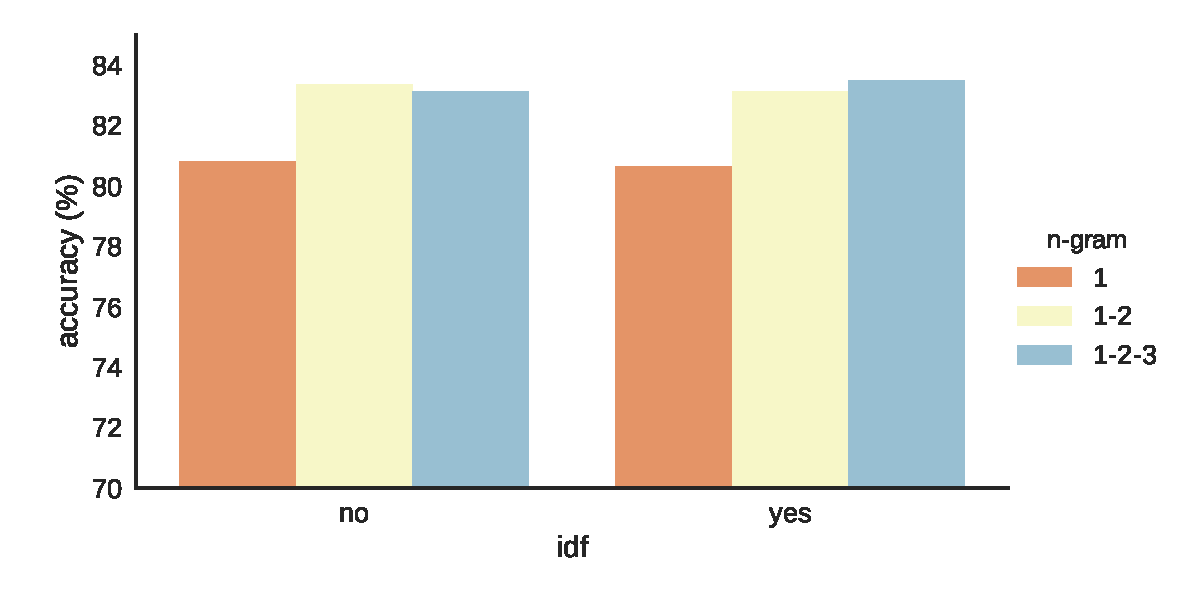
\includegraphics[width=0.9\linewidth]{imag/idf.pdf}
    \caption{Accuracies of logistic regression using bags of words as input.}
    \label{fig:my_label}
\end{figure}

We fed this baseline data to a logistic regression classifier with  $L_2$-regularization. The accuracy for each of the input features (1-grams, 1-grams and 2-grams or 1-grams, 2-grams and 3-grams with and without tf-idf weighting) are given in Figure \ref{fig:my_label}. The model was trained using 95\% of the data while validating it in the remaining 5 \% of the samples. We  notice that the baseline performance in this classification problem is already reasonably high the occurrence of simple words is already quite a good predictor for assigning sentiment to tweets. Moreover, the adding of higher features only seems to increase the performance marginally (1\% for the tf-idf regularization and 3\% for the 1,2,3-gram addition). Similar results were obtained with a single-layer neural network with a softmax activation. Actually, by defining the polarity of a word by the frequency of usage of that given word within a positive tweet (1 if only used within positive tweets, 0 if only within negative ones),this last result becomes quite understandable:


\begin{figure}[h]
    \centering
    \begin{subfigure}[b]{0.25\textwidth}
        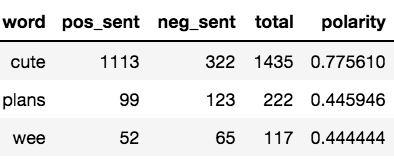
\includegraphics[scale=0.5]{imag/pos.png}
        \caption{}
        \label{pos}
    \end{subfigure}%
    \begin{subfigure}[b]{0.25\textwidth}
        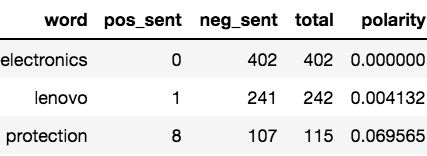
\includegraphics[scale=0.54]{imag/neg.png}
        \caption{}
        \label{neg}
    \end{subfigure}
    \begin{subfigure}[b]{0.5\textwidth}
        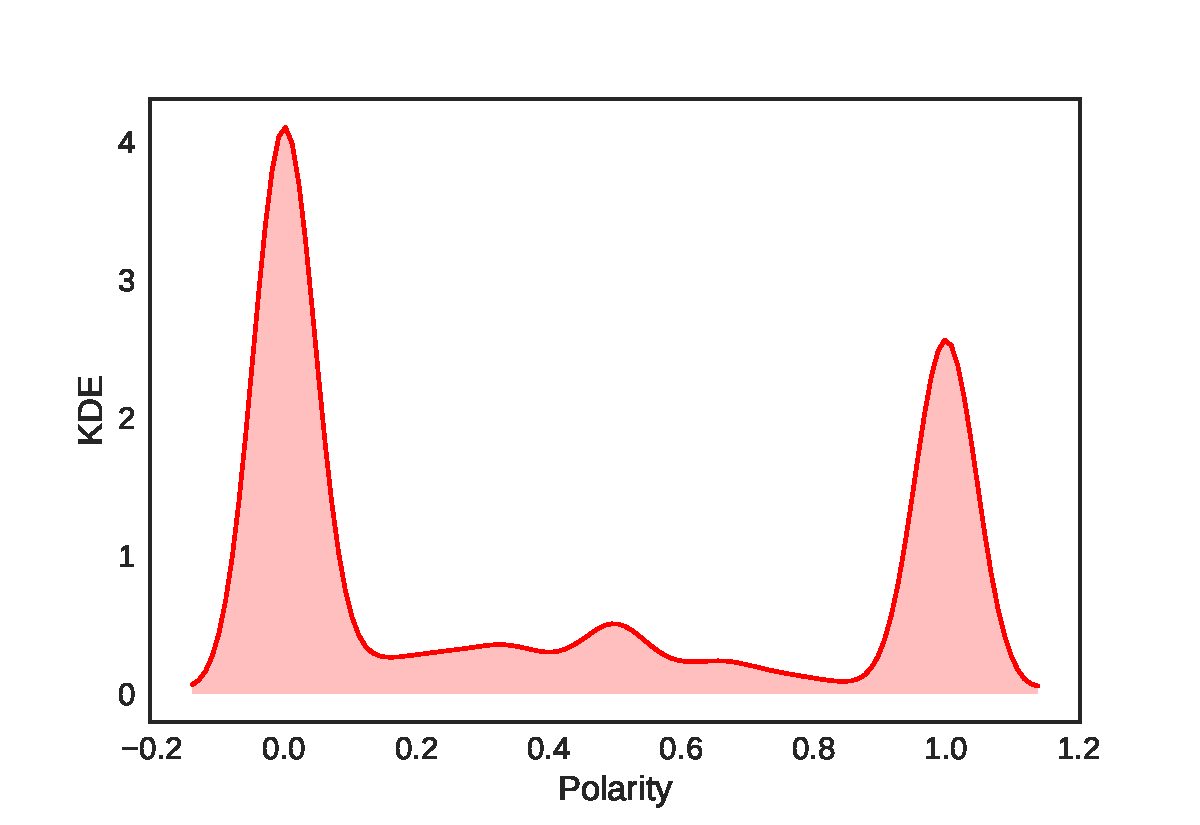
\includegraphics[scale=0.4]{imag/kde_polarity.pdf}
        \caption{}
        \label{polarity1}
    \end{subfigure}
    \caption{a: Top 3 positive polarity words , b: Top 3 negative polarity words, c: polarity density distribution over the observed vocabulary}
    \label{polarity}
\end{figure}

Hence, as we can see in Figure \ref{polarity}, most words are clearly associated to a particular polarity which significantly eases any prediciton task using atomic words features such as BOW. 
We now proceed  to explore how higher level features as well as deeper and more complex learning models might enhance our ability to predict sentiment in the provided dataset.

\subsection{Deep representations}
Since the seminal paper of Mikolov, there has been a growing interest in word embedding methods. Through the latter, words are projected in a lower dimensional dense vector space via a hidden layer of a neural network  (word2vec) or as an output of some optimization problem on the word co-ocurrence matrix (GloVe). 
In both cases, the learned representation tries to capture the different word contexts in which a given a word can appear in, hence enabling, that words in similar context will be embedded close to each other in the representation space. The main advantage of choosing this deeper representation is the dimensionality of the resulting data: every word will now be represented by a dense vector in $\mathbb{R}^D$ where $D$ is the dimension of the embedding. We are specifically relying on two separate sets of pre-trained embeddings, trained respectivelly GloVe and skip-gram with negative sampling (wordvec).
\begin{description}
\item[GloVe pre-trained embeddings:] We rely on a pre-trained set of word embeddings published by the Stanford NLP group. These are trained with a corpus of 2 billions tweets containing around 1.2 millions words covering the quasi-totality of the words in our cleansed vocabulary (words that aren't were filtered out, $D=25$).
\item[Word2Vec pre-trained embeddings:] Unlike the released GloVe dataset, most of the word2vec learned embeddings were trained using news corpus datasets. We hence relied on a dataset released by the NLP group at Ghent's University $D=400$). As in the aforementioned case, most of the encountered words in our dataset were already present in the pre-trained embedding's vocabulary.
\end{description}
These deep representations enable us to build a word representation for all the words in our vocabulary. Some level of aggregation is however needed in order to compute a representation of the tweets that can be fed to a classifier during the learning phase. Different treatments are considered and included. In the first case, tweets are padded to a maximal length of $K_{\text{max}}=35$ words and the GloVe embeddings for each of the words are concatenated together via ther Keras \verb+Embedding+ layer functionality. In the second case, defined for the word2vec embedding, the feature representation for each tweet is obtained by summing over each of the embedding dimensions across all words. 

\section{Classification Models}
Before actually starting to study model performances it's interesting to visualize the dataset in order to check whether there are some clearly observable patterns the algorithms should recognize. We therefore start off my mapping the dense embedding vectors of our tweets to a 2D space using the MultiCore TSNE package. Figure \ref{input} shows the visualization of labeled tweets embedded with the aforementioned word2vec pre-trained model. We can notice the clear absence of any delimiting barrier between positive and negative tweets as clusters of positive and negative tweets seem to overlap in the TSNE mapping space. It is therefore interest to introduce more complex models in order to deal with these higher-level features.\\

\begin{figure}[h]
    \centering
    \begin{subfigure}[b]{0.5\textwidth}
        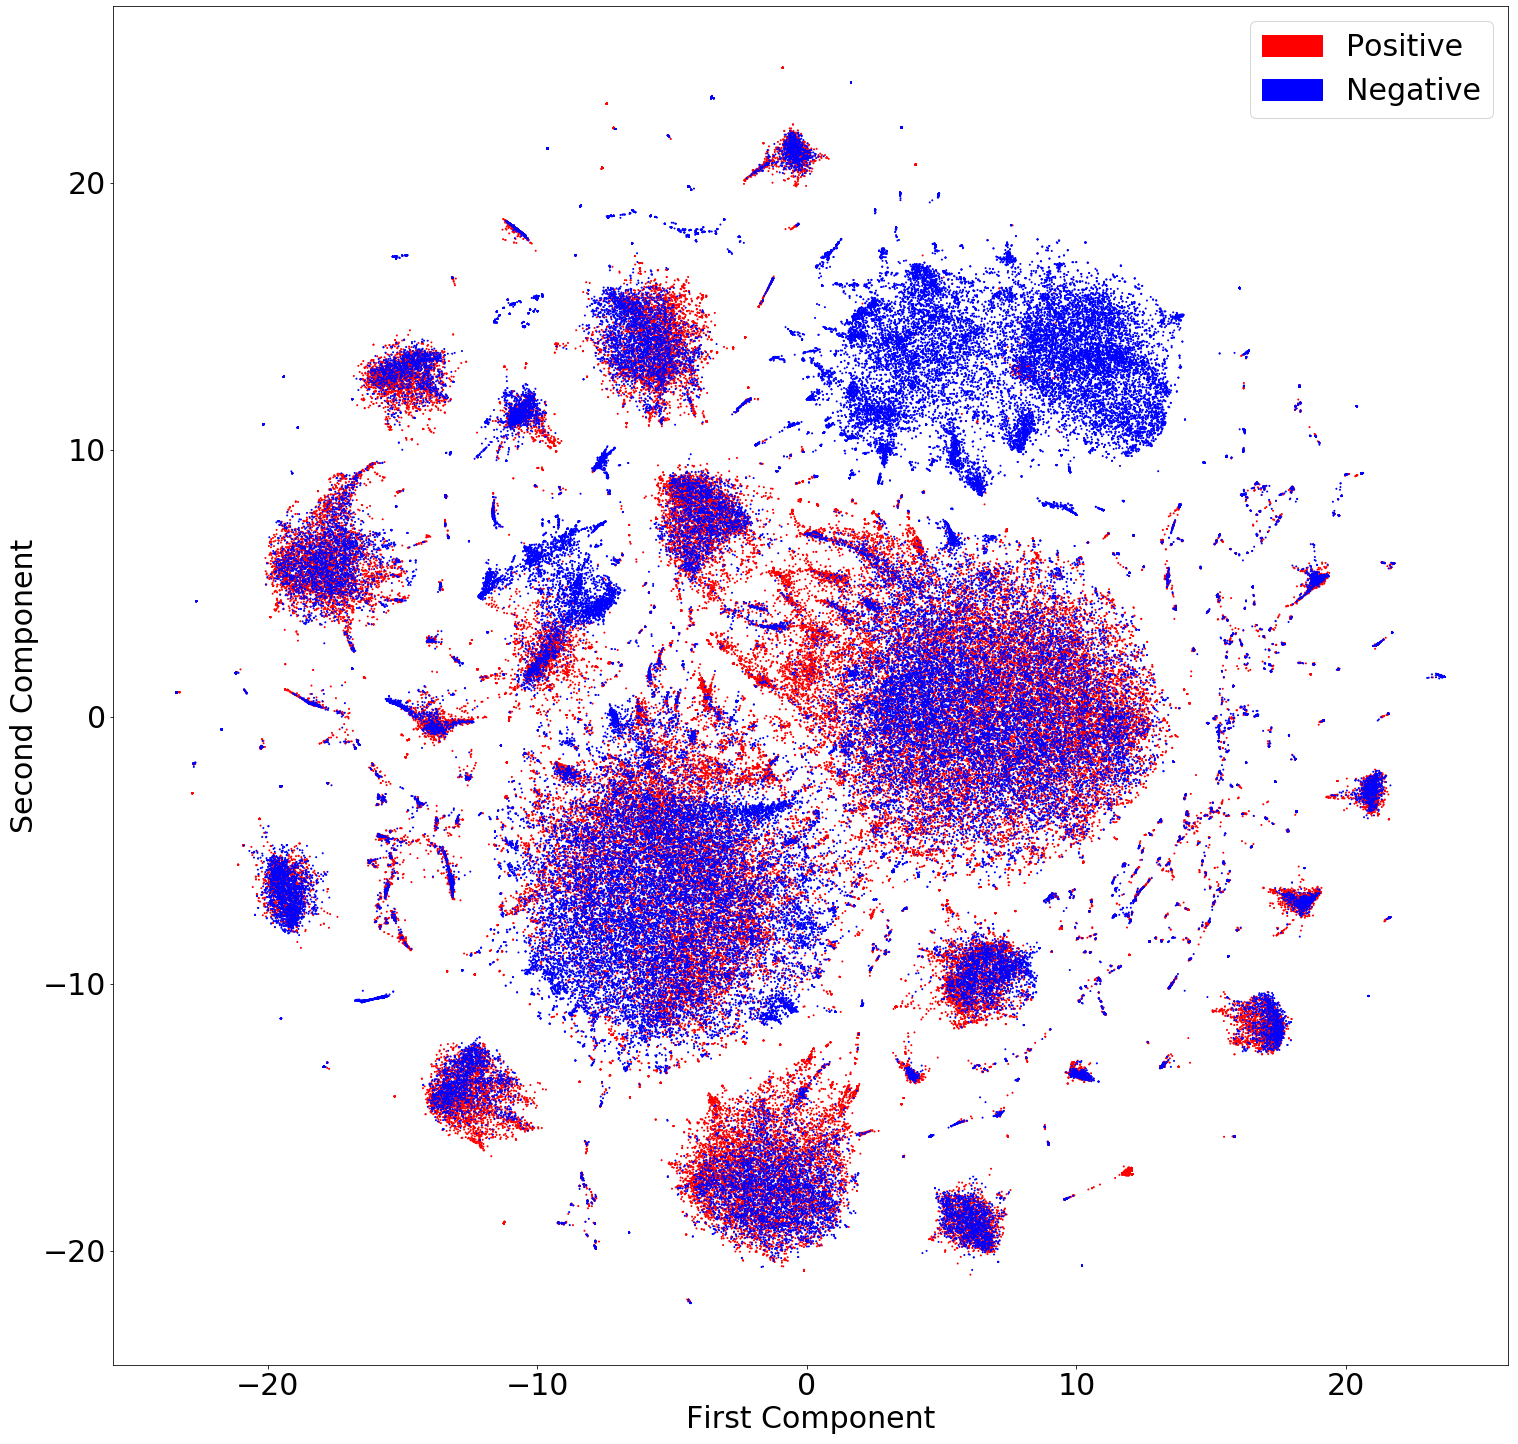
\includegraphics[scale=0.15]{imag/tweets_tsne.png}
        \caption{Input}
        \label{input}
    \end{subfigure}
    \begin{subfigure}[b]{0.5\textwidth}
        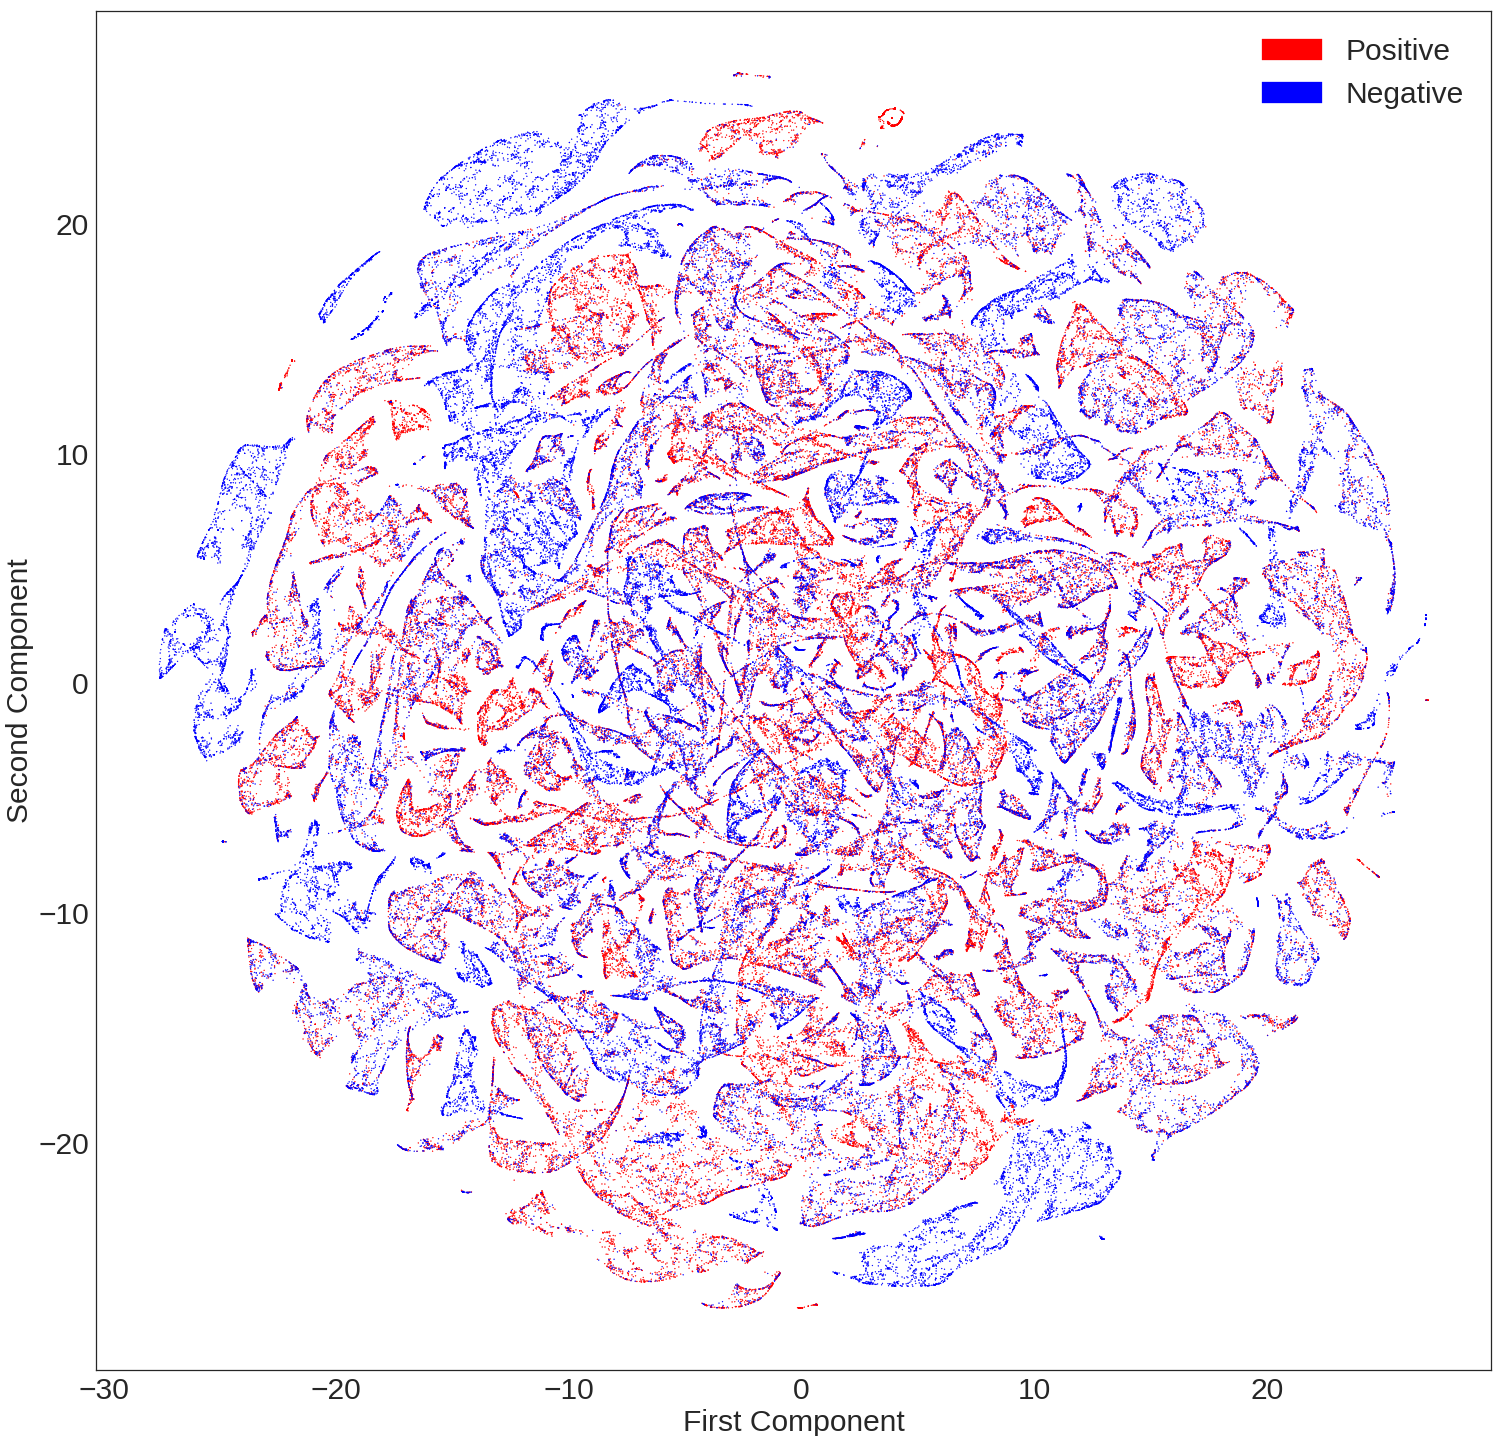
\includegraphics[scale=0.15]{imag/non_tweets_tsne.png}
        \caption{Hidden Layer}
        \label{hidden}
    \end{subfigure}
    \caption{TSNE visualization of embedded tweets by polarity through the network}
    \label{Corr}
\end{figure}

Once the feature engineering step is done, we set out to try different classifiers in order to examine which is best suited for our classifcation problem. Experiments were done with Random Forest, XGBoost, Character Level  LSTM, Deep Neural Networks as well as Convolutional Neural Networks. Given the non-finetuned performance of all these methods on an initial run, we focused on exploring the two latter for our final classification run. \\
Mainly known for their recent success in image recognition problems, CNNs have also become a widespread tool in many NLP tasks. We train a CNN on our GloVe emebeddings where each tweets is represented as a tensor of dimensions  $D_{\text{GloVe}}\times K_{\text{max}}$ by stacking convolutional layers with max-pooling layers (in order to introduce word-interaction features in the network) with a fully connected layer and and a sigmoid activation function to predict class probabilities. \\
A separate deep neural network (DNN) was applied to the word2vec embedding data by stacking densely connected layers. CNNs were in this case no longer useful as the sense of word ordering disappeared when the embedded vectors of each word were averaged. It is actually interesting to see how the progressive introduction of non linear functions (ReLU) in the network allows to generate increasingly separable custer of samples as we can see in Figure \cite{hidden}, where TSNE was applied to the output of the central hidden layer of the DNN. Netowrk architectures are summed up below:




\subsection{Results}


As we are performing a binary classification, we set the loss function to binary crossentropy. We also use the Adam optimizer, described as very efficient for binary classification.

For the training, we observed than epochs after the $2^{nd}$ do not add much value to our accuracy. All different combination of layers led us to accuracies between 85\% and 86\%.
The best results were obtained thanks to the following model : The embedding layer then a convolution1D with 256 filters of length 7 then MaxPooling1D(pool length = 5) then a convolution1D with 128 filters of length 5 then MaxPooling1D(pool length = 3) then a convolution1D with 64 filters of length 5 then MaxPooling1D(pool length = 2) 



All different combination of layers led us to accuracies between 85\% and 86\%.
\section{Other Stuff}
\subsection{Aggregation of several models}

As many of our models had reasonably high but different results, we thought than an average or a vote between different would perform best than every single model. Instead of a simple average, we chose to implement a classifier, which takes as features the outputs of all our different models. We tried several approaches for this purpose : 
\begin{table}[h]
\begin{center}
\begin{tabular}{|c|c|c|c|}
\hline
Model & accuracy \\
\hline
Random Forests & 81.60\% \\
\hline
AdaBoostClassifier & 86.280\% \\
\hline
Logistic regression & 86.540\% \\
\hline

\end{tabular}
\label{classifier}
\caption{Accuracies of final classifiers to aggregate our best models.}
\end{center}
\end{table}


\section{Conclusion}

\end{document}